\documentclass{standalone}
\usepackage{tikz}
\usepackage{graphicx}
\usepackage{xcolor}
\usepackage{amsmath}


\newcommand{\memgrid}[9]{ %TODO
  \begin{scope}[shift={(#1, #2)}]%
    \def\boxwidth{#3}
    \def\addrwidth{#4}
    \def\sizewidth{#5}
    \def\descwidth{#6}
    \def\height{#7}
    \def\lowaddr{#8}
    \def\highaddr{#9}
    %\def\size{#10}
    %\def\description{#11}

    \draw[thick] (0, 0) rectangle (\boxwidth, -\height);
    \draw (\addrwidth, 0) -- (\addrwidth, -\height);
    \draw (\addrwidth+\addrwidth, 0) -- (\addrwidth+\addrwidth, -\height);
    \draw (\addrwidth+\addrwidth+\sizewidth, 0) -- (\addrwidth+\addrwidth+\sizewidth, -\height);

    \node[anchor=mid, align=center] at (\addrwidth/2, -\height/2) {\textbf{\lowaddr}};
    \node[anchor=mid, align=center] at (\addrwidth+\addrwidth/2, -\height/2) {\textbf{\highaddr}};
    %\node[anchor=mid, align=center] at ((\addrwidth+\addrwidth+\sizewidth/2), -\height/2) {\text{\size}};
    %\node[anchor=mid, align=center] at ((\addrwidth+\addrwidth+\sizewidth+\descwidth/2), -\height/2) {\text{\description}};

  \end{scope}
}

\newcommand{\memgridtwo}[7]{
  \def\xsize{#3}
  \def\y{#4}
  \def\xdesc{#5}
  \def\size{#6}
  \def\description{#7}
  \begin{scope}[shift={(#1, #2)}]
    \node[anchor=mid, align=center] at (\xsize, -\y) {\text{\size}};
    \node[anchor=mid, anchor=north, 
	  align=left, text width=8cm, 
	  font=\scriptsize,
	  inner sep=0pt] at (\xdesc, -\y+1.25) {\description};
  \end{scope}
}
\begin{document}

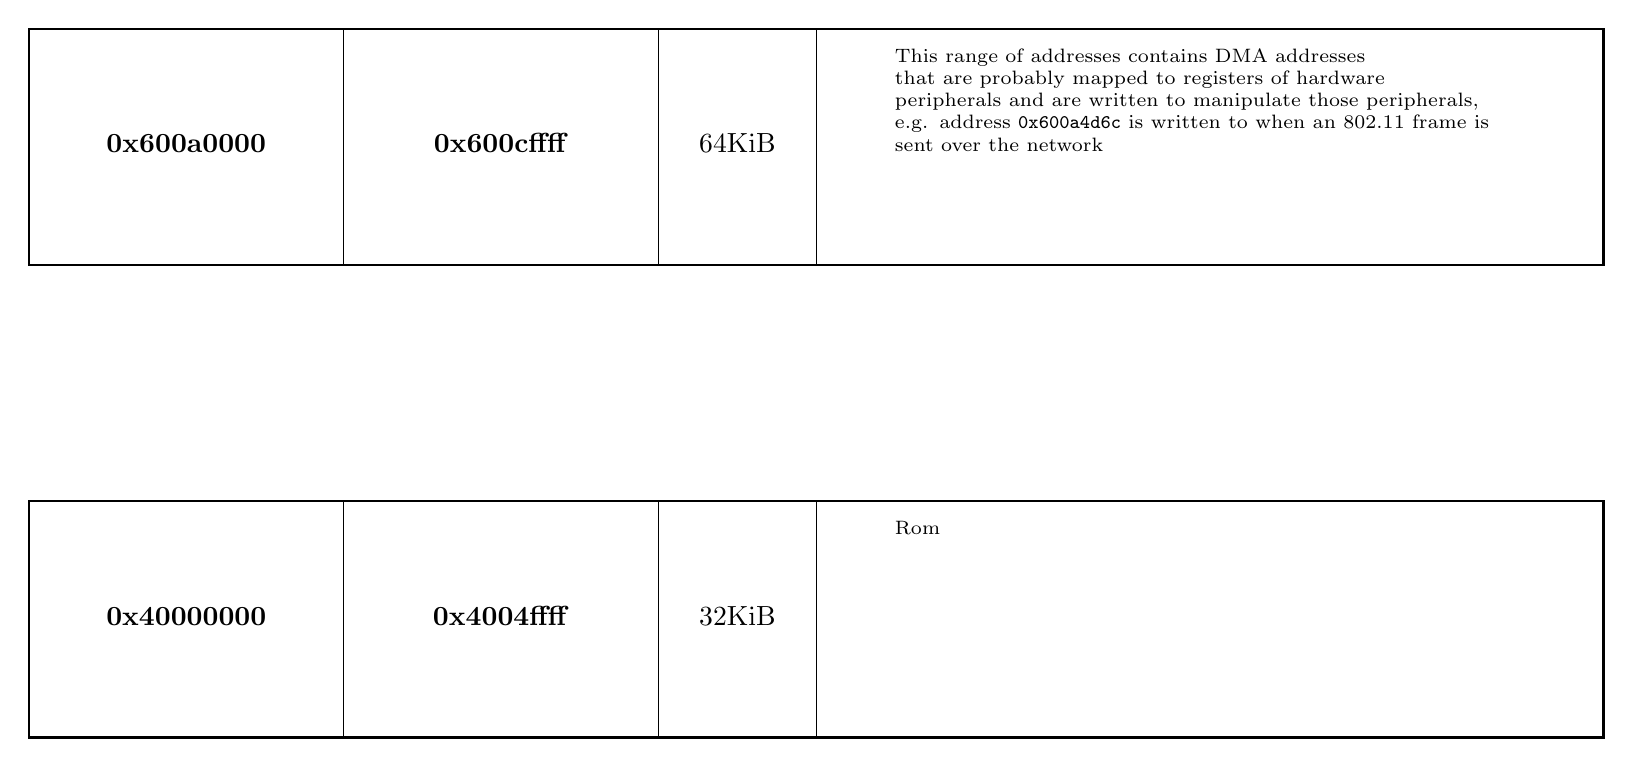
\begin{tikzpicture}

\def\descperiph{
This range of addresses contains DMA addresses \\
that are probably mapped to registers of hardware \\
peripherals and are written to manipulate those peripherals,\\ 
e.g.  address \texttt{0x600a4d6c} is written to when an 802.11 frame is \\ 
sent over the network
}
\memgrid{0}{0}{20}{4}{2}{10}{3}{0x600a0000}{0x600cffff}
\memgridtwo{0}{0}{4+4+1}{1.5}{15}{64KiB}{\descperiph}

\memgrid{0}{-6}{20}{4}{2}{10}{3}{0x40000000}{0x4004ffff}
\memgridtwo{0}{-6}{4+4+1}{1.5}{15}{32KiB}{Rom}

\end{tikzpicture}


\end{document}
